\documentclass{beamer}

\mode<presentation>
{
  \usetheme{default}
  \usecolortheme{default}
  \usefonttheme{default}
  \setbeamertemplate{navigation symbols}{}
  \setbeamertemplate{caption}[numbered]
}

\usepackage[utf8]{inputenc}
\usepackage{ngerman}
\usepackage{lmodern}
\usepackage{amsthm}
\usepackage{amssymb}
\usepackage{amsmath}
\usepackage{mathtools}
\usepackage{graphicx}
\usepackage{paralist}

\newtheorem{satz}{Satz}
%\newtheorem{definition}[satz]{Definition}
%\newtheorem{lemma}[satz]{Lemma}
\newtheorem{proposition}{Proposition}
%Create a new theorem by writing \newtheorem{How to call this type of theorem}[satz]{What should be written}. Make sure to keep "satz" to ensure consecutive numeration.
% %  Variablen Definition...............
\newcommand*{\R}{k[X_{1},\ldots,X_{n}]}
\newcommand*{\indx}[2]{{#1}_{#2}}
\newcommand*{\potx}[2]{{#1}^{#2}}
\newcommand*{\N}{\mathbb{N}_0}
\newcommand*{\hf}[1]{$\prescript{a}{}{HF}_{#1}$}
\newcommand*{\hp}[1]{$\prescript{a}{}{HP}_{#1}$}
\newcommand*{\kette}[2]{$1\leq {#1}_1<{#1}_2<{#1}_3<...<{#1}_{#2}\leq n$}
\newcommand*{\dkette}[2]{${#1}_1,{#1}_2,{#1}_3,\ldots,{#1}_{#2} \in \mathbb{N}$}
\newcommand*{\Rr}[2]{$ k[X_{{#1}_{1}},\ldots,X_{{#1}_{#2}}]$}
%\newcommand*{\hf}{}
\newcommand*{\ideal}{$I$}


\title{Dimension von Varietäten}
\date{\today}
\author{Yvan Ngumeteh \and Emma Ahrens}

\begin{document}

\begin{frame}
	\begin{figure}[ht]
		\centering
		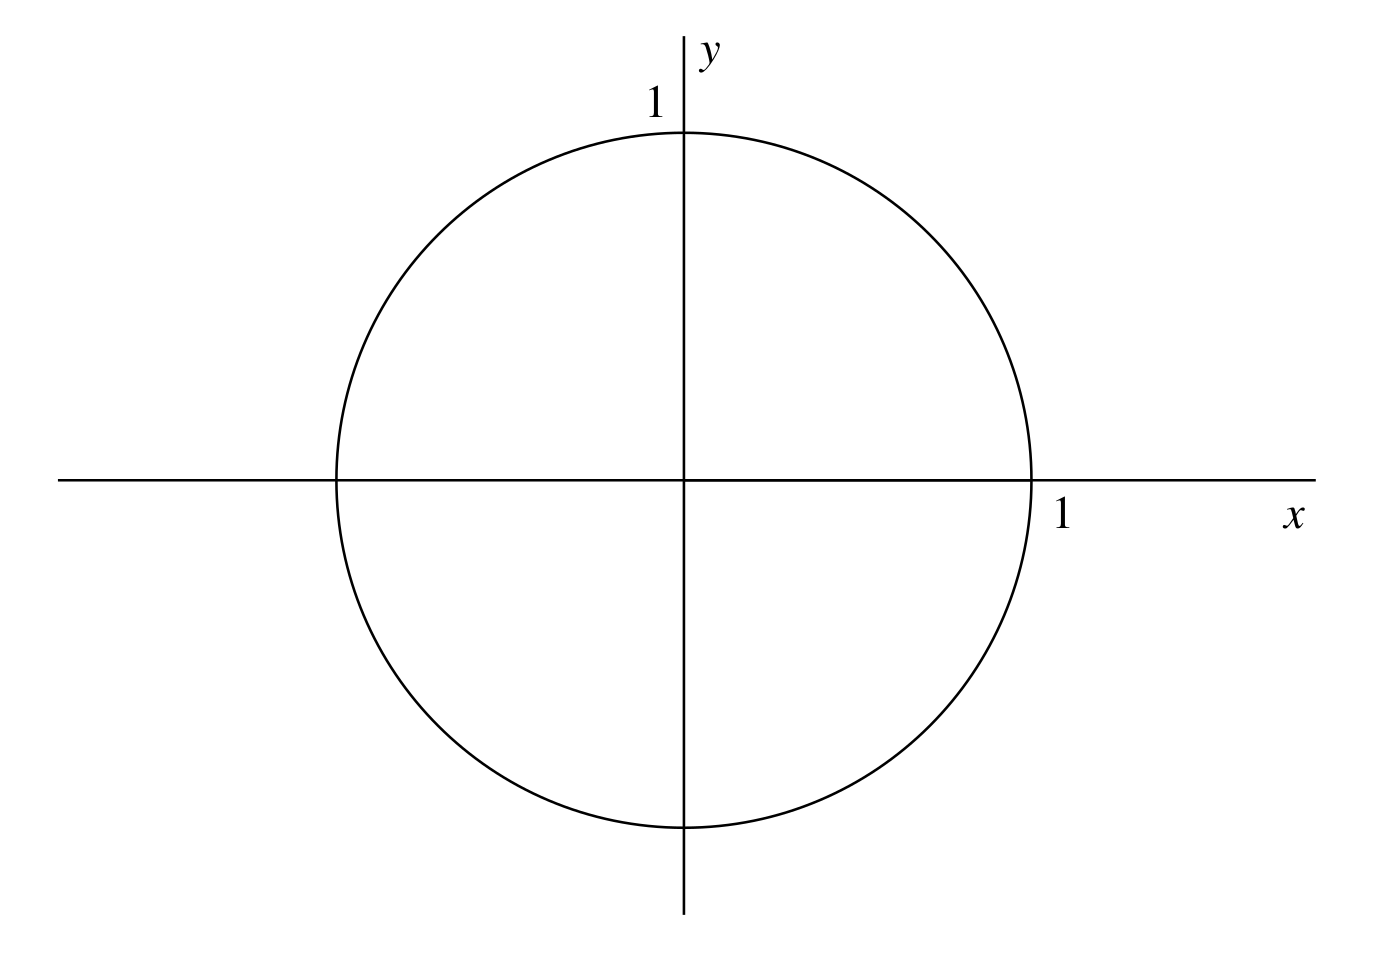
\includegraphics[width=.75\linewidth]{circle.png}
		\caption{Die Varietät \(V(X^2 + Y^2 -1)\) aus \cite{CLOS}}
		\label{circle}
	\end{figure}
\end{frame}

\begin{frame}
	\begin{figure}[ht]
		\centering
		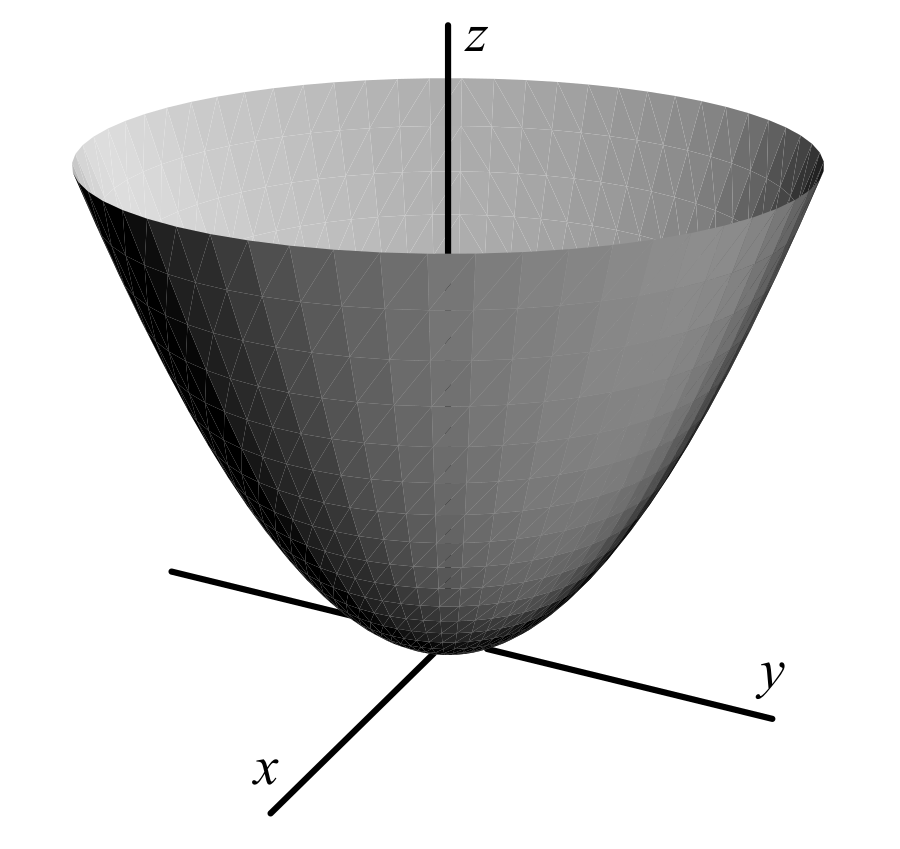
\includegraphics[width=.5\linewidth]{paraboloid.png}
		\caption{Das elliptische Paraboloid \(V(Z - X^2 -Y)\) aus \cite{CLOS}}
		\label{paraboloid}
	\end{figure}
\end{frame}

\begin{frame}
	\begin{lemma} \label{1.2.3}
	Sei \(I \subseteq \R\) ein Ideal, das von einer Menge G von Monomen erzeugt wird. Dann liegt
	ein Polynom \(f \in \R\) in I genau dann, wenn für jeden Term \(a_{j}X^{\alpha_{j}}\) von f ein
	\(g \in G\) existiert, welches \(a_{j}X^{\alpha_{j}}\) teilt.
	\end{lemma}
\end{frame}

\begin{frame}
	\begin{lemma} \label{1.2.4}
	Sei \((g_{i})_{i \geq 1}\) eine Folge von Monomen in \(\R\) mit \(g_{1} \succeq g_{2} \succeq
	\ldots\) für eine Monomialordnung \(\preceq\). Dann existiert ein \(r \in \mathbb{N}\) mit 
	\(g_{n} = g_{r}\) für alle \(n \geq r\). 
	\end{lemma}
\end{frame}

\begin{frame}
	\begin{proposition}[Divisionsalgorithmus] \label{1.2.5}
	Sei \(\preceq\) eine Monomialordnung und \(f, f_{1}, \ldots, f_{s} \in \R\) nicht null. Dann
	gilt \begin{displaymath} f = \sum_{i=1}^{s} h_{i}f_{i}\; + r, \end{displaymath} mit
	\(r, h_{1}, \ldots, h_{s} \in \R\) und \(LT(h_{i}f_{i} \preceq LT(f)\) für alle \(h_{i} \neq 0
	\) und \(r = 0\) oder kein Term von r wird durch ein \(LT(f_{i})\) geteilt für \(i \in
	\underline{s}\).
	\end{proposition}
\end{frame}

\begin{frame}
	\begin{satz} \label{1.2.8}
	Sei \(\{0\} \neq I \subseteq \R\) ein Ideal und \(\preceq\) eine Monomialordnung auf
	\(\mathbb{N}^{n}_{0}\). Sei G eine Gröbnerbasis von I mit I = (G). Dann ist eine k-Basis von 
	\(\R/I\) gegeben durch die Restklassen von \(X^{\alpha}\) mit
	\begin{displaymath}
	\alpha \in C(I) := \{\alpha \in \mathbb{N}^{n}_{0}\; |\;\; LT(g) \nmid X^{\alpha}\; \forall g 
	\in G\}.
	\end{displaymath}
	\end{satz}
\end{frame}

\begin{frame}
	\begin{figure}[ht]
		\centering
		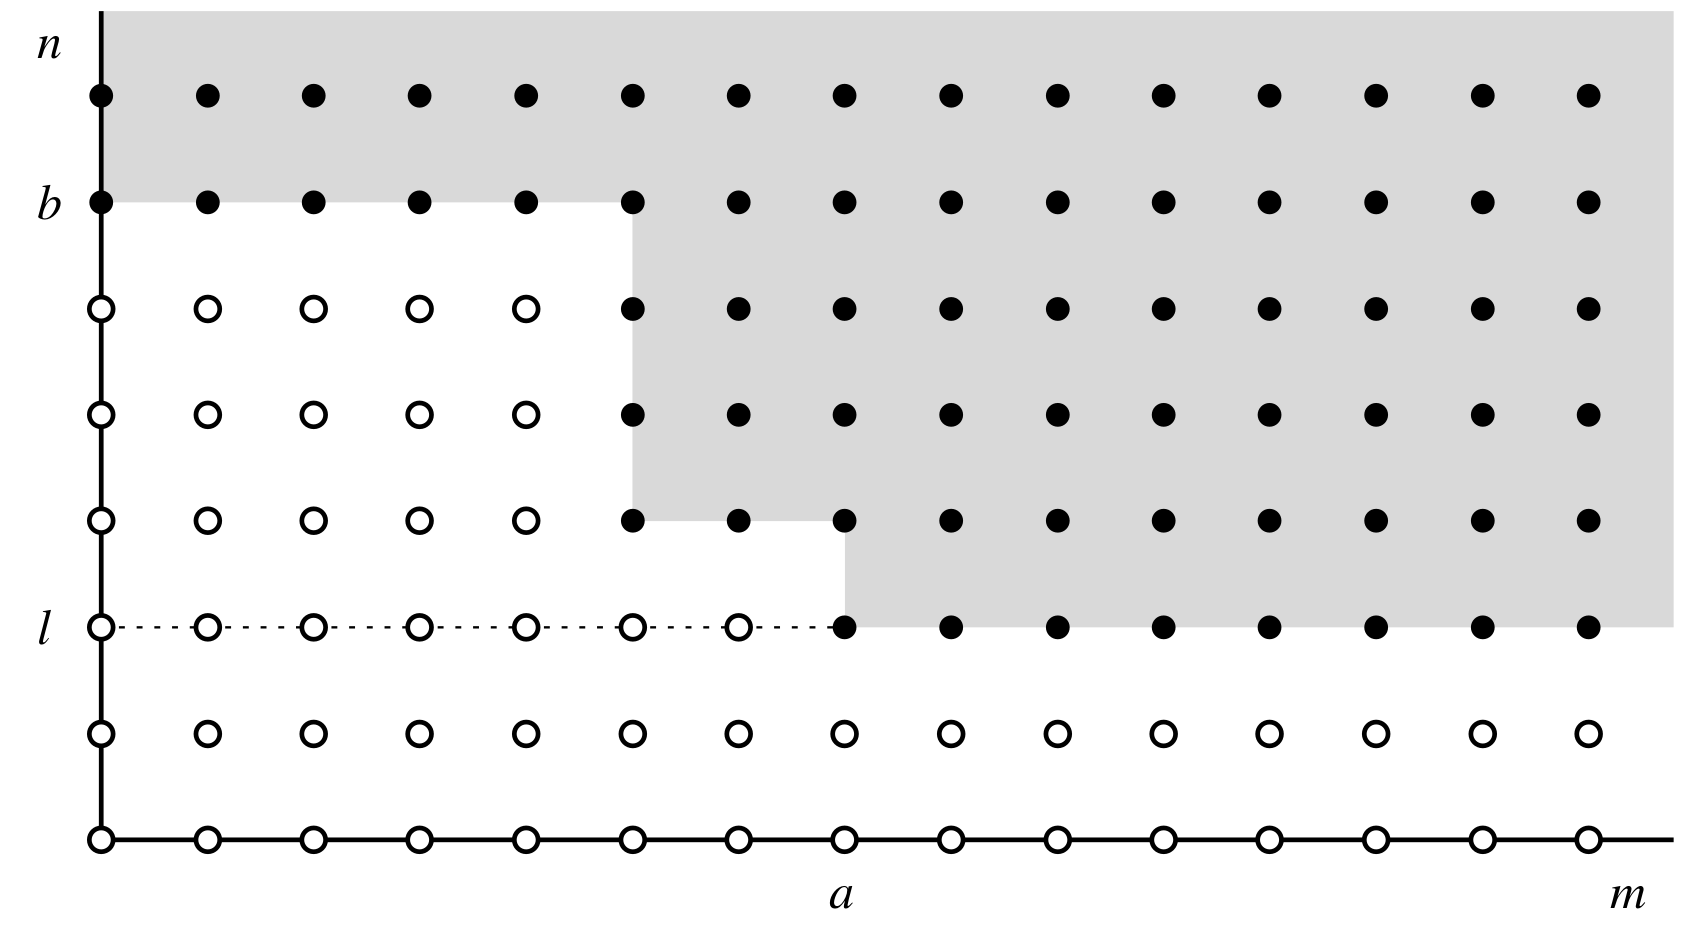
\includegraphics[width=.75\linewidth]{Dots.png}
		\caption{Anschauliche Darstellung von \(\R/I\) aus \cite{CLOS}}
		\label{dots}
	\end{figure}
\end{frame}

\begin{frame}
	\begin{definition} \label{1.2.11}
	Sei \(I \subseteq \R\) ein Ideal und \(s \in \mathbb{N}_{0}\). Dann definiere \(I_{\leq s} :=
	I \cap \R_{\leq s}\). Nun gilt, dass \(\R_{\leq s}\) ein endlich dimensionaler Vektorraum über
	k  mit \(I_{\leq s}\) als Teilraum ist. Wir können die Funktion \begin{displaymath}
	\prescript{a}{}{HF}_{I} : \mathbb{N}_{0} \rightarrow \mathbb{N}_{0}, \quad s \mapsto
	dim_{k}(\R_{\leq s}/I_{\leq s})	\end{displaymath} definieren, die (affine) Hilbertfunktion
	von I genannt wird.
	\end{definition}
\end{frame}

\begin{frame}
	\begin{lemma}[Macaulay] \label{1.2.13}
	Sei \(\preceq\) eine gradierte lexikographische Monomialordnung und \(I \subseteq \R\) ein
	Ideal. Dann ist \(\prescript{a}{}{HF}_{I}(s) = \prescript{a}{}{HF}_{LT(I)}(s)\) für alle
	\(s \in \mathbb{N}_{0}\).
	\end{lemma}
\end{frame}

\begin{frame}
	\begin{satz}
		\label{1.2.14}
		Sei  \ideal $\unlhd$ $\R$, dann existiert ein eindeutiges Polynom \hp{I}(t) $\in \mathbb{Q}[t]$ (t ist eine Variable) und $\indx{s}{0}\geq0$,  sodass \hp{I}(s)=\hf{I}(s)= $\indx{dim}{k}$ ($\indx{\R}{\leq s}$/$\indx{I}{\leq s}$), für alle $ s\geq\indx{s}{0}$. Weiterhin besitzt \hp{I}(t) folgende Eigenschaften:	
	\end{satz}
	\begin{compactenum}
		\item[a)] Der Grad von \hp{I}(t) ist der größte $d \in \mathbb{N}$, sodass es \dkette{i}{d} mit \kette{i}{d} existieren und $I\cap k[X_{{i}_{1}},\ldots,X_{{i}_{d}}]={\emptyset}$.
		\item[b)] Sei $d=grad(\textnormal{\hp{I}})$. Dann gilt \hp{I}(t)=$\sum_{k=0}^{d} \indx{a}{k}t^k$ mit $\indx{a}{k}d! \in \mathbb{Z}, \forall k\in \underline{\indx{d}{0}}$ und $\indx{a}{d}d!>0$\\
	\end{compactenum}
\end{frame}

	% %
\begin{frame}
	\begin{definition}
		Sei $V\subset k^n$ eine algebraische Menge und \hp{I(V)}(t) ist das Hilbert-Polynom von $I(V)\unlhd\R$ (nach Satz \ref{1.2.14} ist wohldefiniert und eindeutig). Für $V\neq\emptyset$ (d.h. $I(V)\neq\R$), wird die Dimension definiert als 
		
		\begin{displaymath}
		dim(V)=grad(\textnormal{\hp{I(V)}}).
		\end{displaymath}
		Eine etwas handlichere Charakterisierung ist nach Satz \ref{1.2.14} durch:
		
		\begin{displaymath}
		dim(I(V))=\max{\{d\in\underline{n}:\exists{\,} 1\leq\indx{i}{1}<\ldots<\indx{i}{d}\leq n \textnormal{ mit } I\cap K[\indx{X}{\indx{i}{1}},\ldots,\indx{X}{\indx{i}{d}}]=\{0\} \}}
		\end{displaymath}
		gegeben.\\
	\end{definition}
\end{frame}
	% %

\begin{frame}
	\begin{proposition}
		Sei $V\subseteq k^n$ algebraisch und $V=\bigcup\limits_{i\in\underline{r}}\indx{V}{i}$ eine Zerlegung in irreduziblen Komponenten (vgl. Proposition 1.1.11). Dann gilt
		\begin{displaymath}
		dim(V)=\max{\{dim(\indx{V}{i}):i\in\underline{r}\}}
		\end{displaymath}
	\end{proposition}
\end{frame}

\begin{frame} 
	\begin{definition}
		Sei $A$ eine $k-$Algebra (kommutativer, assoziativer $k-$Algebra mit 1). Man nennt $\indx{a}{1},\ldots,\indx{a}{m}\in A$ algebraisch unabhängig, falls 
		\begin{displaymath}
		\forall \;F\in k[\indx{X}{1},\ldots,\indx{X}{m}]\setminus\{0\} \;\textnormal{gilt}\; F(\indx{a}{1},\ldots,\indx{a}{m})\neq0.
		\end{displaymath}
		Man definiert
		\begin{displaymath}
		\indx{\partial}{k}(A):=\sup{\{m\geq0:\;\exists\; m \;\textnormal{algebraisch unabhängige Elemente in}\; A\}}
		\end{displaymath}
		Bemerkung: Falls A ein Körper ist, dann nennt man $\indx{\partial}{k}(A)$ der transcendenz Grad von $A$ über $k$.\\
	\end{definition}
\end{frame}
	% %

\begin{frame}
	\begin{proposition}
		Sei $A:=\R/I$ mit $I\unlhd\R$ ein echtes Ideal. Dann gilt $grad(\textnormal{\hp{I}})=\indx{\partial}{k}(A)$. Ist $A$ weiterhin einen Integrietätsbereich $(IB)$ und $K$ ist der Quotienten-Körper von $A$, dann gilt
		\begin{displaymath}
		grad(\textnormal{\hp{I}})=\indx{\partial}{k}(A)=\indx{\partial}{k}(K).
		\end{displaymath}
		Insbesondere gilt $dim(V)=\indx{\partial}{k}(A[V])$ für jede nicht-leere algebraische $V\subset k^n$.\\
	\end{proposition}
\end{frame}
	% %

\begin{frame}
	\begin{lemma}
		Sei $V\subseteq k^n$ irreduzible algebraischer Menge und $W\subseteq V$ abgeschlossenen Teilmenge. Dann gilt $dim(W)<dim(V)$, falls $W$ echte Teilmenge von $V$ ist.
	\end{lemma}
\end{frame}

\begin{frame}
	\begin{thebibliography}{99}
		\bibitem{CLOS}
		\textsc{Cox}, David; \textsc{Little}, John; \textsc{O'Shea}, Donal:
		\newblock \emph{Ideals, Varieties, and Algorithms}.
		\newblock Third Edition
		\newblock Springer-Verlag, 2007
	\end{thebibliography}
\end{frame}

\end{document}
